\documentclass[mathserif]{beamer}

%\usetheme{LCOM}
\usetheme{Madrid}
\usepackage{hyperref}
\usepackage{listings}
\usepackage{graphicx}
\usepackage[english]{babel}
\usepackage[utf8]{inputenc}
\usepackage[T1]{fontenc}
\usepackage{booktabs}
\usepackage{amsmath,amssymb,amsthm,mathrsfs,amsfonts,dsfont}
\usepackage{adjustbox}
\usepackage{array}
\usepackage{longtable}
\usepackage{psfrag}
\usepackage{caption}
\usepackage{placeins}
\usepackage{subfig}
\usepackage{multirow}
\usepackage[absolute,overlay]{textpos}

\newcommand{\wait}{\vfill}
%\newcommand{\wait}{\pause}
	
\DeclareMathAlphabet\mathbfcal{OMS}{cmsy}{b}{n}
\newcommand\blfootnote[1]{%
	\begingroup
	\renewcommand\thefootnote{}\footnote{#1}%
	\addtocounter{footnote}{-1}%
	\endgroup
}

\setbeamertemplate{frametitle continuation}[from second][]

\title[Visual Light Communication - VLC]{Visual Light Communication - VLC} 
\author[Vinícius Lagrota]{Autor: Vinícius Lagrota Rodrigues da Costa\\
	Orientador: Moisés Vidal Ribeiro}
\institute[UFJF]{Programa de Pós-Graduação em Engenharia Elétrica\\
	Universidade Federal de Juiz de Fora}
%\date{15 de dezembro 2017}
\date{\today}

\begin{document}

\begin{frame}
\maketitle 
\end{frame}

\begin{frame}
\frametitle{Outlines}
\small
\tableofcontents
\end{frame}

%--------------------------------------------------------------------------
\section{Introduction}
\begin{frame}
\frametitle{Outlines}
	\small
	\tableofcontents[currentsection]
\end{frame}
%--------------------------------------------------------------------------
\subsection{Overview}
%-----------------------
\begin{frame}
	\frametitle{Introduction}
	\framesubtitle{Overview}

	Optical Wireless Communication (OWC): \wait
	\begin{itemize}		
		\item Free Space Optical (FSO).
		\begin{itemize}
			\item Infrared.
			\item Point-to-point.
			\item 750–1600 nm. \wait
		\end{itemize}
		\item \textbf{Visual Light Communication (VLC)}.
		\begin{itemize}
			\item 350–750 nm. \wait
		\end{itemize}
		\item Ultraviolet Communication  (UVC).
		\begin{itemize}
			\item 200–280 nm. \wait
		\end{itemize}
	\end{itemize}
\end{frame}	

%-----------------------
\subsection{Spectrum}
%-----------------------
\begin{frame}
\frametitle{Introduction}
\framesubtitle{Spectrum}
	\begin{figure}
		\centering
		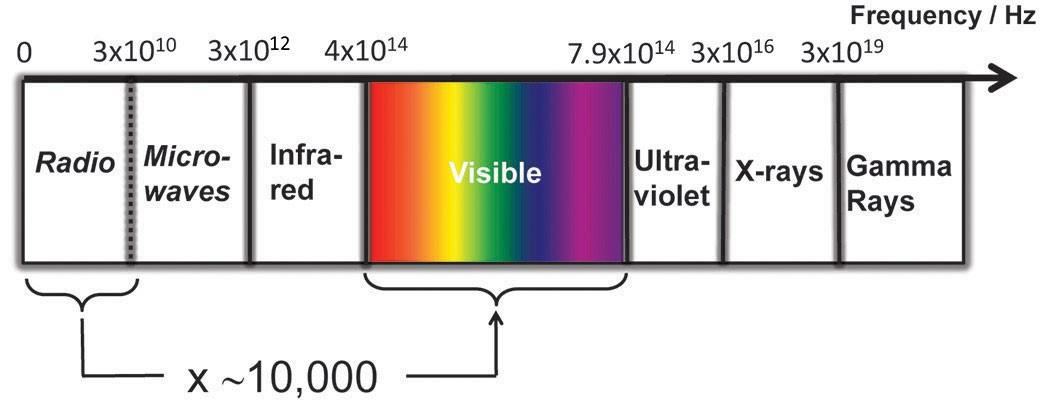
\includegraphics[width=\linewidth]{figuras/spectrum}
		\caption{Spectrum.}
		\label{fig:spectrum}
	\end{figure}
\end{frame}	

%--------------------------------------------------------------------------
\subsection{Motivation}
%--------------------------------------------------------------------------
\begin{frame}
\frametitle{Introduction}
\framesubtitle{Motivation}
	\begin{itemize}
		\item VLC spectrum 10000 times greater than RF spectrum. \wait
		\item Crowded RF spectrum. \wait
		\item High energy efficiency. \wait
		\item Security
			\begin{itemize}
				\item Restricted environment.
				\item Aircrafts, hospitals. \wait
			\end{itemize}
		\item Availability.
	\end{itemize}

\end{frame}	

%--------------------------------------------------------------------------
\subsection{Disadvantages}
%--------------------------------------------------------------------------
\begin{frame}
\frametitle{Introduction}
\framesubtitle{Disadvantages}
	\begin{itemize}
		\item Sunlight $\Rightarrow$ full spectrum $\Rightarrow$ interference. \wait
		\item Point-to-multipoint managing $\Rightarrow$ public places.
		\begin{itemize}
			\item Security of devices. \wait
		\end{itemize}
		\item Illumination system with communication capabilities $\Rightarrow$ not otherwise.
		\begin{itemize}
			\item Dimming, illumination control, oscillation. \wait
		\end{itemize}
	\end{itemize}	
\end{frame}	

%--------------------------------------------------------------------------
\subsection{Applications}
%--------------------------------------------------------------------------
\begin{frame}
\frametitle{Introduction}
\framesubtitle{Applications}
	\begin{itemize}
		\item Hospitals. \wait
		\item Petrochemical industry. \wait
		\item Aircrafts. \wait
		\item Traffic control. \wait
		\item Safe environments \wait
	\end{itemize}
\end{frame}	

%--------------------------------------------------------------------------
\subsection{Link}
%--------------------------------------------------------------------------
\begin{frame}
\frametitle{Introduction}
\framesubtitle{Link}
	Line-of-Sight (LOS)
	\begin{itemize}
		\item Directed.
		\item Non-directed.
	\end{itemize}

	\wait
	Non line-of-Sight (NLOS)
	\begin{itemize}
		\item Directed.
		\item Non-directed.
	\end{itemize}

	\begin{textblock*}{7cm}(5cm,3cm) % {block width} (coords)
		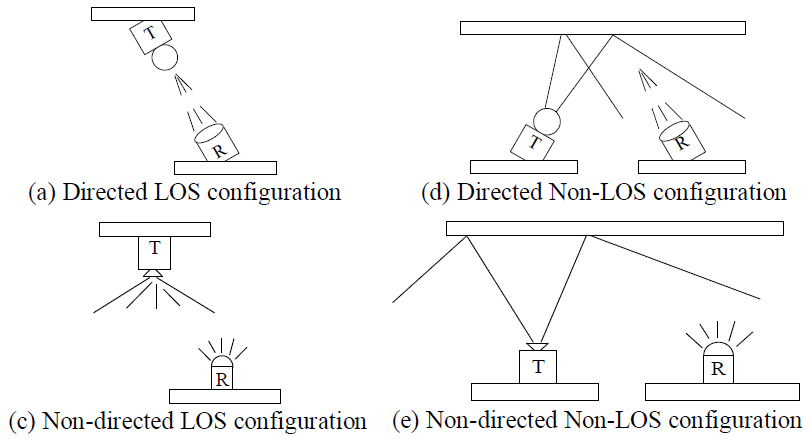
\includegraphics[width=7cm]{figuras/link.png}
	\end{textblock*}
\end{frame}	



%--------------------------------------------------------------------------
\section{Modulation}
\begin{frame}
\frametitle{Outlines}
	\small
	\tableofcontents[currentsection]
\end{frame}
%--------------------------------------------------------------------------

\begin{frame}
\frametitle{Modulation}
Single Carrier Modulation (SCM):
\begin{itemize}
	\item On-off keying (OOK).
	\item Pulse Width Modulation (PWM).
	\item Pulse-amplitude modulation (M-PAM). \wait
\end{itemize}

OFDM.
\begin{itemize}
	\item DC biased OFDM (DCO-OFDM).
	\item Polar OFDM (P-OFDM). \wait
\end{itemize}

Colour Domain Modulation:
\begin{itemize}
	\item \textbf{Colour Shift Keying (CSK).}
	\item Colour intensity modulation (CIM). \wait
\end{itemize}	
\end{frame}	

\begin{frame}
\frametitle{Modulation}
\begin{figure}
\centering
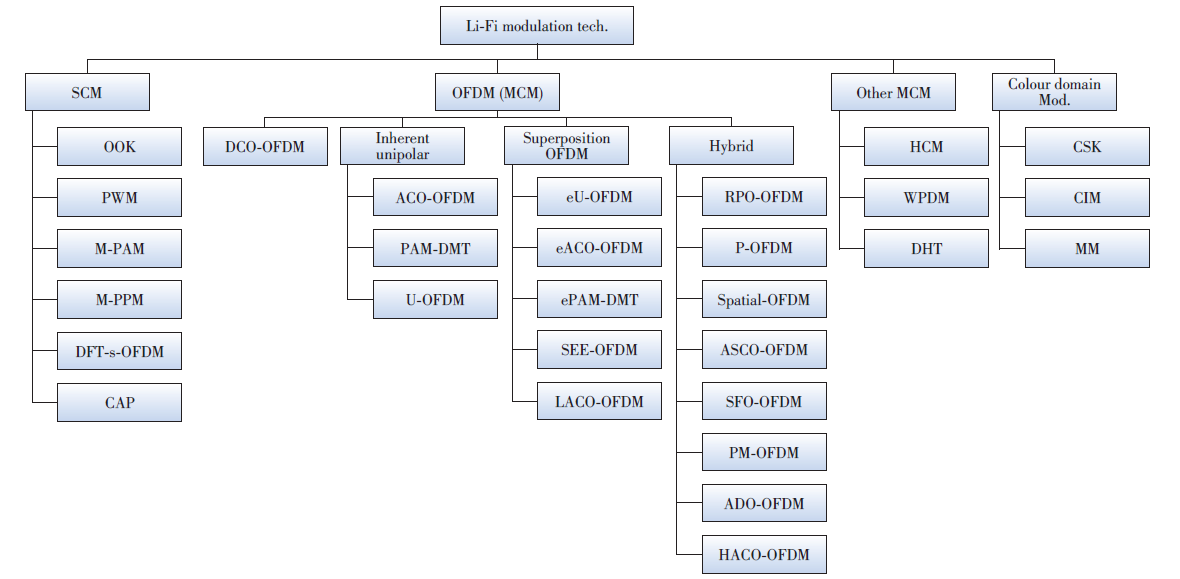
\includegraphics[width=\linewidth]{figuras/modulation}
\caption{Modulation schemes.}
\label{fig:modulation}
\end{figure}
\end{frame}	

%--------------------------------------------------------------------------
\section{Transceptor}
\begin{frame}
\frametitle{Outlines}
	\small
	\tableofcontents[currentsection]
\end{frame}
%--------------------------------------------------------------------------
%\subsection{Transmitter}
%-----------------------
\begin{frame}
\frametitle{Transceptor}
%\framesubtitle{Transmitter}
	Transmitter:
	\begin{itemize}
		\item Laser Diodes (LD).
		\begin{itemize}
			\item Coherent light source $\Rightarrow$ same phase.
		\end{itemize}
		\item L\textbf{ight Emitting Diode (LED)}
		\begin{itemize}
			\item Incoherent light source $\Rightarrow$ different phases.
			\item Single-colour LED.
			\item Multi-colour LED.
		\end{itemize}
	\end{itemize}
	\wait
	
	Receiver:
	\begin{itemize}
		\item Photodetector.
		\begin{itemize}
			\item Photomultipliers.
			\item Photoconductors.
			\item Phototransistors.
			\item \textbf{Photodiodes.}
		\end{itemize}
	\end{itemize}

	\begin{textblock*}{4cm}(8.5cm,2.5cm) % {block width} (coords)
		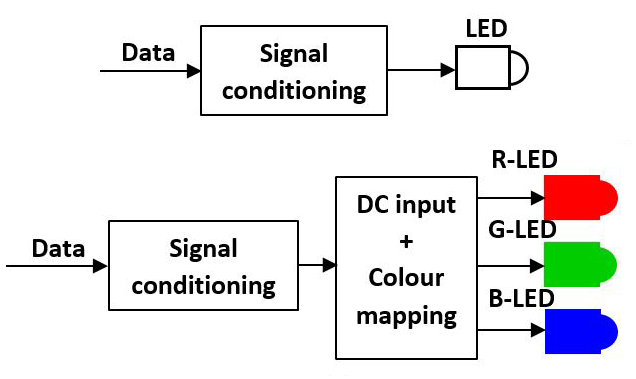
\includegraphics[width=4cm]{figuras/led.png}
	\end{textblock*}

	\begin{textblock*}{2cm}(9.6cm,5.8cm) % {block width} (coords)
		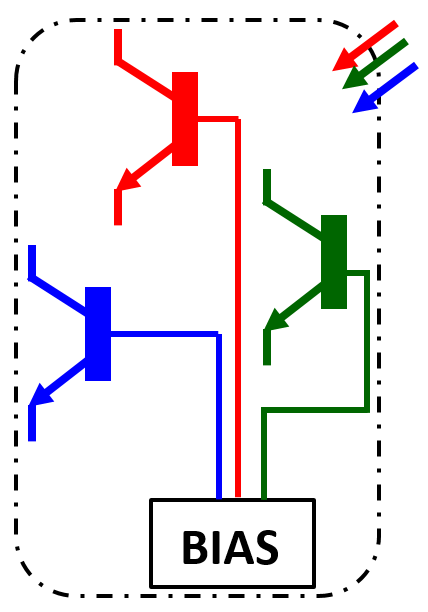
\includegraphics[width=2cm]{figuras/pd.png}
	\end{textblock*}
\end{frame}


%--------------------------------------------------------------------------
\section{Equations}
\begin{frame}
\frametitle{Outlines}
	\small
	\tableofcontents[currentsection]
\end{frame}
%--------------------------------------------------------------------------
%\subsection{Transmitter}
%-----------------------
\begin{frame}
\frametitle{System diagram}
	\begin{figure}
		\centering
		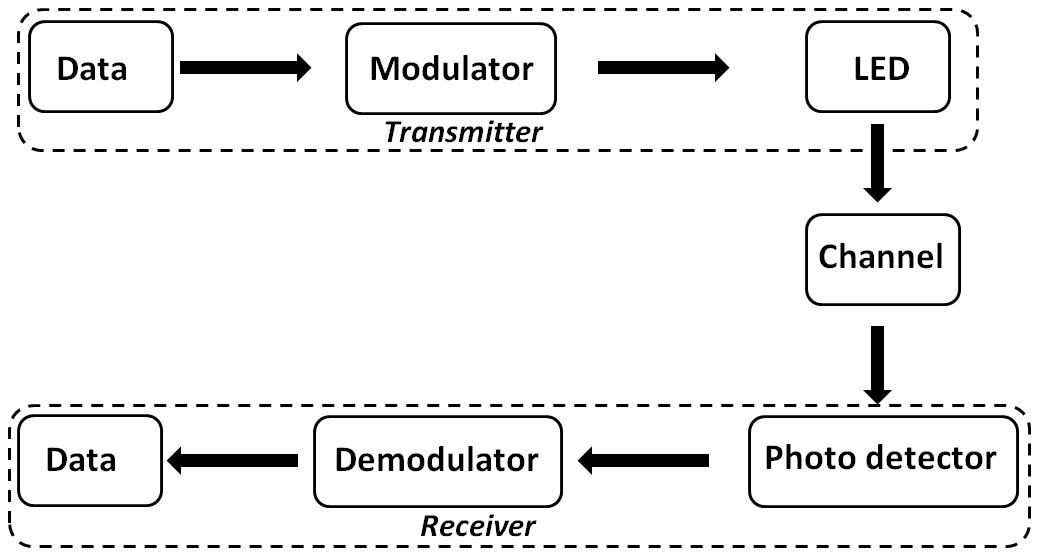
\includegraphics[width=\linewidth]{figuras/transceptor}
		\caption{System diagram.}
		\label{fig:transceptor}
	\end{figure}
\end{frame}

\begin{frame}
\frametitle{Equations}
	VLC system corrupted by AWGN:
	\begin{equation}
		{\mathbf{Y}_v} = {\mathbf{H}_v}{\mathbf{S}_v} + {\mathbf{N}_v}
	\end{equation}
	$\mathbf{Y}_v$: received sets of symbols.\\
	$\mathbf{S}_v$: transmitted sets of symbols.\\
	$\mathbf{H}_v$: channel frequency response.\\
	$\mathbf{N}_v$: channel noise.\\
	Under de influence of a hypothetical thermal noise:
	\begin{equation}
	{\mathbf{Y}_v} = {{\chi _0}\mathbf{H}_v}{\mathbf{S}_v} + {\mathbf{N}_v}
	\end{equation}
	${\chi _0}$: thermal noise ${\rm{(0 }} \le {\rm{ }}{\chi _0}{\rm{ }} \le {\rm{ 1)}}$.\\
	 ${\chi _0} = 0 \Rightarrow$ absence of light.\\
	 ${\chi _0} = 1 \Rightarrow$ presence of light.
\end{frame}


\begin{frame}
\frametitle{System diagram}
	\begin{figure}
		\centering
		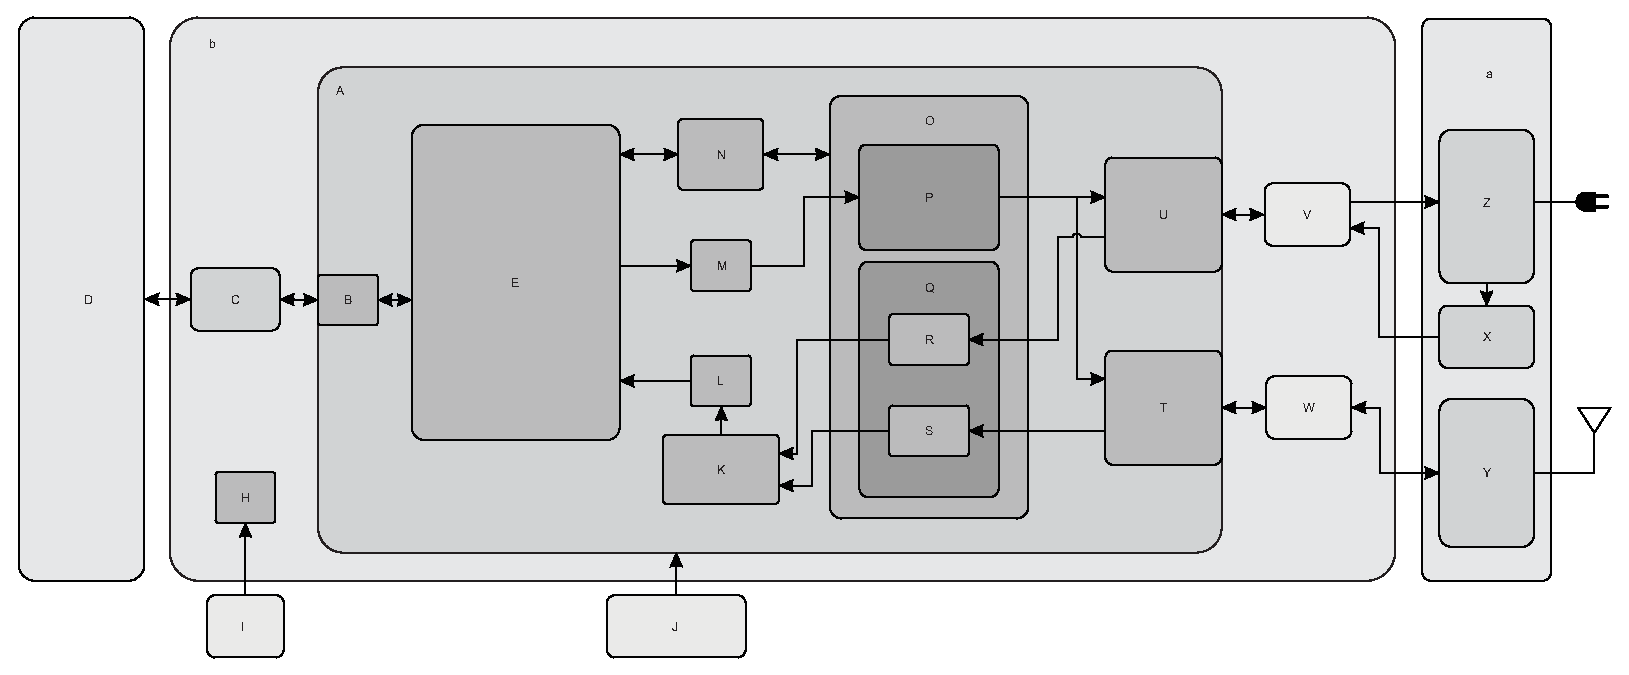
\includegraphics[width=\linewidth]{figuras/block_diagram}
		\caption{Block diagram.}
		\label{fig:block_diagram}
	\end{figure}
\end{frame}

\begin{frame}
\frametitle{Noise}
	Source:
	\begin{itemize}
		\item Sunlight.
		\item Incandescent light.
		\item Fluorescent light.
	\end{itemize}
	Type:
	\begin{itemize}
		\item Thermal noise.
		\item Shot noise.
	\end{itemize}
\end{frame}

%------------------------------------------------
\begin{frame}[noframenumbering]
	\vfill
	\centering
	\Huge{Thank you!}
	\vfill
\end{frame}

\end{document}
